\documentclass[1p]{elsarticle_modified}
%\bibliographystyle{elsarticle-num}

%\usepackage[colorlinks]{hyperref}
%\usepackage{abbrmath_seonhwa} %\Abb, \Ascr, \Acal ,\Abf, \Afrak
\usepackage{amsfonts}
\usepackage{amssymb}
\usepackage{amsmath}
\usepackage{amsthm}
\usepackage{scalefnt}
\usepackage{amsbsy}
\usepackage{kotex}
\usepackage{caption}
\usepackage{subfig}
\usepackage{color}
\usepackage{graphicx}
\usepackage{xcolor} %% white, black, red, green, blue, cyan, magenta, yellow
\usepackage{float}
\usepackage{setspace}
\usepackage{hyperref}

\usepackage{tikz}
\usetikzlibrary{arrows}

\usepackage{multirow}
\usepackage{array} % fixed length table
\usepackage{hhline}

%%%%%%%%%%%%%%%%%%%%%
\makeatletter
\renewcommand*\env@matrix[1][\arraystretch]{%
	\edef\arraystretch{#1}%
	\hskip -\arraycolsep
	\let\@ifnextchar\new@ifnextchar
	\array{*\c@MaxMatrixCols c}}
\makeatother %https://tex.stackexchange.com/questions/14071/how-can-i-increase-the-line-spacing-in-a-matrix
%%%%%%%%%%%%%%%

\usepackage[normalem]{ulem}

\newcommand{\msout}[1]{\ifmmode\text{\sout{\ensuremath{#1}}}\else\sout{#1}\fi}
%SOURCE: \msout is \stkout macro in https://tex.stackexchange.com/questions/20609/strikeout-in-math-mode

\newcommand{\cancel}[1]{
	\ifmmode
	{\color{red}\msout{#1}}
	\else
	{\color{red}\sout{#1}}
	\fi
}

\newcommand{\add}[1]{
	{\color{blue}\uwave{#1}}
}

\newcommand{\replace}[2]{
	\ifmmode
	{\color{red}\msout{#1}}{\color{blue}\uwave{#2}}
	\else
	{\color{red}\sout{#1}}{\color{blue}\uwave{#2}}
	\fi
}

\newcommand{\Sol}{\mathcal{S}} %segment
\newcommand{\D}{D} %diagram
\newcommand{\A}{\mathcal{A}} %arc


%%%%%%%%%%%%%%%%%%%%%%%%%%%%%5 test

\def\sl{\operatorname{\textup{SL}}(2,\Cbb)}
\def\psl{\operatorname{\textup{PSL}}(2,\Cbb)}
\def\quan{\mkern 1mu \triangleright \mkern 1mu}

\theoremstyle{definition}
\newtheorem{thm}{Theorem}[section]
\newtheorem{prop}[thm]{Proposition}
\newtheorem{lem}[thm]{Lemma}
\newtheorem{ques}[thm]{Question}
\newtheorem{cor}[thm]{Corollary}
\newtheorem{defn}[thm]{Definition}
\newtheorem{exam}[thm]{Example}
\newtheorem{rmk}[thm]{Remark}
\newtheorem{alg}[thm]{Algorithm}

\newcommand{\I}{\sqrt{-1}}
\begin{document}

%\begin{frontmatter}
%
%\title{Boundary parabolic representations of knots up to 8 crossings}
%
%%% Group authors per affiliation:
%\author{Yunhi Cho} 
%\address{Department of Mathematics, University of Seoul, Seoul, Korea}
%\ead{yhcho@uos.ac.kr}
%
%
%\author{Seonhwa Kim} %\fnref{s_kim}}
%\address{Center for Geometry and Physics, Institute for Basic Science, Pohang, 37673, Korea}
%\ead{ryeona17@ibs.re.kr}
%
%\author{Hyuk Kim}
%\address{Department of Mathematical Sciences, Seoul National University, Seoul 08826, Korea}
%\ead{hyukkim@snu.ac.kr}
%
%\author{Seokbeom Yoon}
%\address{Department of Mathematical Sciences, Seoul National University, Seoul, 08826,  Korea}
%\ead{sbyoon15@snu.ac.kr}
%
%\begin{abstract}
%We find all boundary parabolic representation of knots up to 8 crossings.
%
%\end{abstract}
%\begin{keyword}
%    \MSC[2010] 57M25 
%\end{keyword}
%
%\end{frontmatter}

%\linenumbers
%\tableofcontents
%
\newcommand\colored[1]{\textcolor{white}{\rule[-0.35ex]{0.8em}{1.4ex}}\kern-0.8em\color{red} #1}%
%\newcommand\colored[1]{\textcolor{white}{ #1}\kern-2.17ex	\textcolor{white}{ #1}\kern-1.81ex	\textcolor{white}{ #1}\kern-2.15ex\color{red}#1	}

{\Large $\underline{12n_{0549}~(K12n_{0549})}$}

\setlength{\tabcolsep}{10pt}
\renewcommand{\arraystretch}{1.6}
\vspace{1cm}\begin{tabular}{m{100pt}>{\centering\arraybackslash}m{274pt}}
\multirow{5}{120pt}{
	\centering
	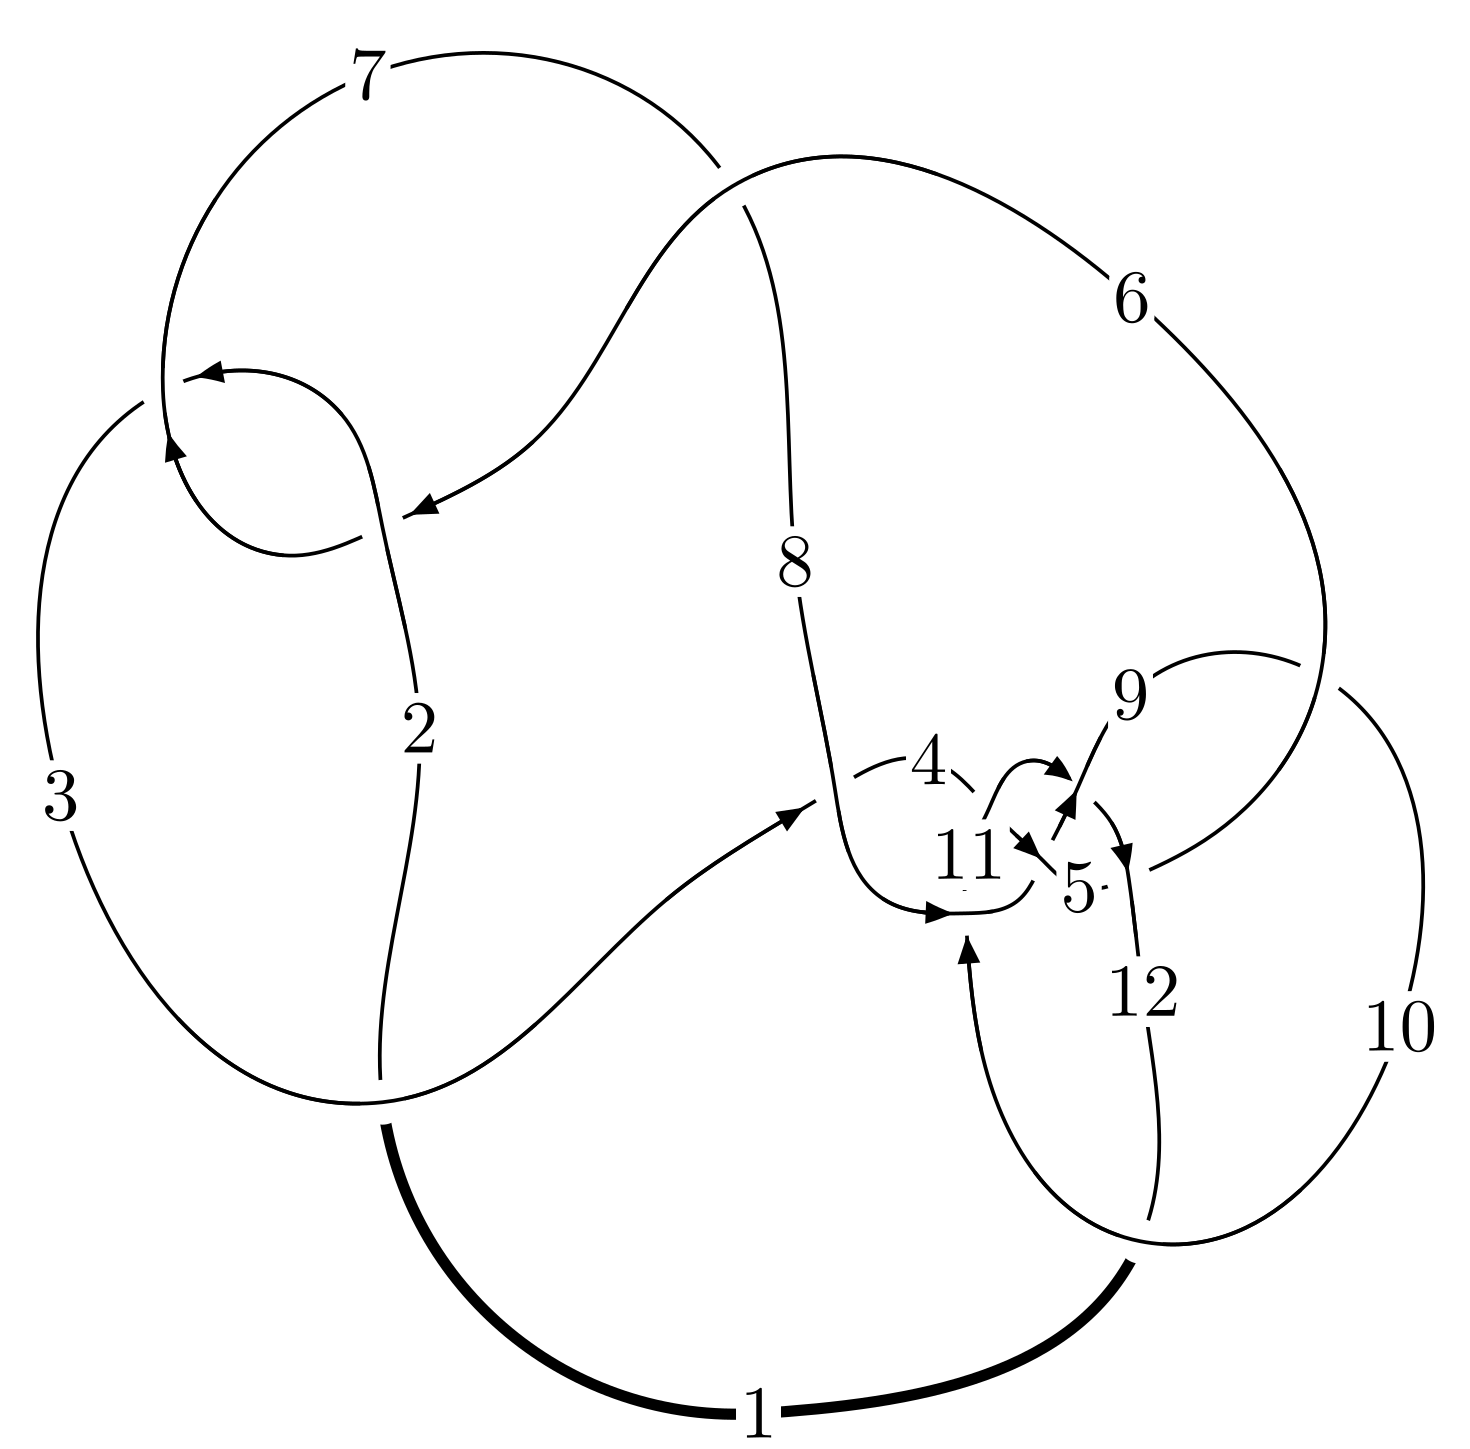
\includegraphics[width=112pt]{../../../GIT/diagram.site/Diagrams/png/2638_12n_0549.png}\\
\ \ \ A knot diagram\footnotemark}&
\allowdisplaybreaks
\textbf{Linearized knot diagam} \\
\cline{2-2}
 &
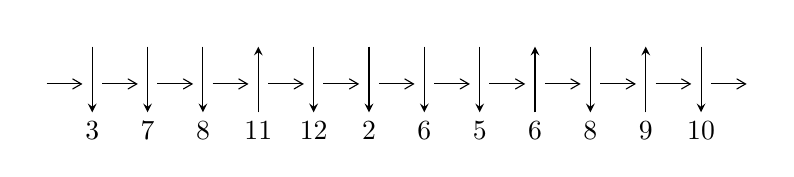
\begin{tikzpicture}[x=20pt, y=17pt]
	% nodes
	\node (C0) at (0, 0) {};
	\node (C1) at (1, 0) {};
	\node (C1U) at (1, +1) {};
	\node (C1D) at (1, -1) {3};

	\node (C2) at (2, 0) {};
	\node (C2U) at (2, +1) {};
	\node (C2D) at (2, -1) {7};

	\node (C3) at (3, 0) {};
	\node (C3U) at (3, +1) {};
	\node (C3D) at (3, -1) {8};

	\node (C4) at (4, 0) {};
	\node (C4U) at (4, +1) {};
	\node (C4D) at (4, -1) {11};

	\node (C5) at (5, 0) {};
	\node (C5U) at (5, +1) {};
	\node (C5D) at (5, -1) {12};

	\node (C6) at (6, 0) {};
	\node (C6U) at (6, +1) {};
	\node (C6D) at (6, -1) {2};

	\node (C7) at (7, 0) {};
	\node (C7U) at (7, +1) {};
	\node (C7D) at (7, -1) {6};

	\node (C8) at (8, 0) {};
	\node (C8U) at (8, +1) {};
	\node (C8D) at (8, -1) {5};

	\node (C9) at (9, 0) {};
	\node (C9U) at (9, +1) {};
	\node (C9D) at (9, -1) {6};

	\node (C10) at (10, 0) {};
	\node (C10U) at (10, +1) {};
	\node (C10D) at (10, -1) {8};

	\node (C11) at (11, 0) {};
	\node (C11U) at (11, +1) {};
	\node (C11D) at (11, -1) {9};

	\node (C12) at (12, 0) {};
	\node (C12U) at (12, +1) {};
	\node (C12D) at (12, -1) {10};
	\node (C13) at (13, 0) {};

	% arrows
	\draw[->,>={angle 60}]
	(C0) edge (C1) (C1) edge (C2) (C2) edge (C3) (C3) edge (C4) (C4) edge (C5) (C5) edge (C6) (C6) edge (C7) (C7) edge (C8) (C8) edge (C9) (C9) edge (C10) (C10) edge (C11) (C11) edge (C12) (C12) edge (C13) ;	\draw[->,>=stealth]
	(C1U) edge (C1D) (C2U) edge (C2D) (C3U) edge (C3D) (C4D) edge (C4U) (C5U) edge (C5D) (C6U) edge (C6D) (C7U) edge (C7D) (C8U) edge (C8D) (C9D) edge (C9U) (C10U) edge (C10D) (C11D) edge (C11U) (C12U) edge (C12D) ;
	\end{tikzpicture} \\
\hhline{~~} \\& 
\textbf{Solving Sequence} \\ \cline{2-2} 
 &
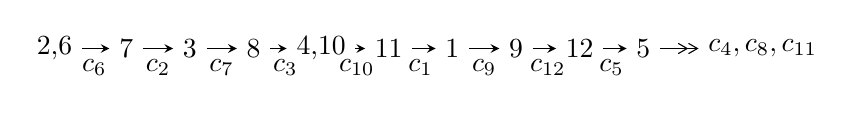
\begin{tikzpicture}[x=23pt, y=7pt]
	% node
	\node (A0) at (-1/8, 0) {2,6};
	\node (A1) at (1, 0) {7};
	\node (A2) at (2, 0) {3};
	\node (A3) at (3, 0) {8};
	\node (A4) at (65/16, 0) {4,10};
	\node (A5) at (41/8, 0) {11};
	\node (A6) at (49/8, 0) {1};
	\node (A7) at (57/8, 0) {9};
	\node (A8) at (65/8, 0) {12};
	\node (A9) at (73/8, 0) {5};
	\node (C1) at (1/2, -1) {$c_{6}$};
	\node (C2) at (3/2, -1) {$c_{2}$};
	\node (C3) at (5/2, -1) {$c_{7}$};
	\node (C4) at (7/2, -1) {$c_{3}$};
	\node (C5) at (37/8, -1) {$c_{10}$};
	\node (C6) at (45/8, -1) {$c_{1}$};
	\node (C7) at (53/8, -1) {$c_{9}$};
	\node (C8) at (61/8, -1) {$c_{12}$};
	\node (C9) at (69/8, -1) {$c_{5}$};
	\node (A10) at (11, 0) {$c_{4},c_{8},c_{11}$};

	% edge
	\draw[->,>=stealth]	
	(A0) edge (A1) (A1) edge (A2) (A2) edge (A3) (A3) edge (A4) (A4) edge (A5) (A5) edge (A6) (A6) edge (A7) (A7) edge (A8) (A8) edge (A9) ;
	\draw[->>,>={angle 60}]	
	(A9) edge (A10);
\end{tikzpicture} \\ 

\end{tabular} \\

\footnotetext{
The image of knot diagram is generated by the software ``\textbf{Draw programme}" developed by Andrew Bartholomew(\url{http://www.layer8.co.uk/maths/draw/index.htm\#Running-draw}), where we modified some parts for our purpose(\url{https://github.com/CATsTAILs/LinksPainter}).
}\phantom \\ \newline 
\centering \textbf{Ideals for irreducible components\footnotemark of $X_{\text{par}}$} 
 
\begin{align*}
I^u_{1}&=\langle 
- u^3- u^2+b,\;a- u,\;u^4+u^3-2 u+1\rangle \\
I^u_{2}&=\langle 
- u^3- u^2+b,\;a- u,\;u^4+u^3+1\rangle \\
I^u_{3}&=\langle 
- u^4+u^3- u^2+b,\;a- u,\;u^6- u^5+u^4+u^3+u^2+u+1\rangle \\
I^u_{4}&=\langle 
- u^5+2 u^4- u^3- u^2+b,\;- u^3+2 u^2+a- u,\;u^6- u^5+u^4+u^3+u^2+u+1\rangle \\
I^u_{5}&=\langle 
- u^4- u^2+2 b- u-2,\;-3 u^5- u^4- u^3+10 a-9 u-8,\;u^6+2 u^5+2 u^4+3 u^2+6 u+5\rangle \\
I^u_{6}&=\langle 
b- u,\;- u^2+a+u,\;u^3- u-1\rangle \\
I^u_{7}&=\langle 
b- u,\;u^2+a- u+1,\;u^3- u^2+1\rangle \\
I^u_{8}&=\langle 
- u^2+b+u,\;a- u,\;u^3- u^2+1\rangle \\
I^u_{9}&=\langle 
b,\;a+1,\;u+1\rangle \\
I^u_{10}&=\langle 
b-1,\;a,\;u-1\rangle \\
\end{align*}\\
\begin{align*}
I^u_{11}&=\langle 
b-1,\;a-1,\;u-1\rangle \\
\\
I^v_{1}&=\langle 
a,\;b-1,\;v+1\rangle \\
\end{align*}
\raggedright * 12 irreducible components of $\dim_{\mathbb{C}}=0$, with total 39 representations.\\
\footnotetext{All coefficients of polynomials are rational numbers. But the coefficients are sometimes approximated in decimal forms when there is not enough margin.}
\newpage
\renewcommand{\arraystretch}{1}
\centering \section*{I. $I^u_{1}= \langle - u^3- u^2+b,\;a- u,\;u^4+u^3-2 u+1 \rangle$}
\flushleft \textbf{(i) Arc colorings}\\
\begin{tabular}{m{7pt} m{180pt} m{7pt} m{180pt} }
\flushright $a_{2}=$&$\begin{pmatrix}0\\u\end{pmatrix}$ \\
\flushright $a_{6}=$&$\begin{pmatrix}1\\0\end{pmatrix}$ \\
\flushright $a_{7}=$&$\begin{pmatrix}1\\u^2\end{pmatrix}$ \\
\flushright $a_{3}=$&$\begin{pmatrix}- u\\- u^3+u\end{pmatrix}$ \\
\flushright $a_{8}=$&$\begin{pmatrix}- u^2+1\\u^2\end{pmatrix}$ \\
\flushright $a_{4}=$&$\begin{pmatrix}-4 u^3- u^2+5 u-3\\3 u^3- u^2-3 u+2\end{pmatrix}$ \\
\flushright $a_{10}=$&$\begin{pmatrix}u\\u^3+u^2\end{pmatrix}$ \\
\flushright $a_{11}=$&$\begin{pmatrix}2 u^3+u^2-2 u+1\\- u^3+u^2+2 u-1\end{pmatrix}$ \\
\flushright $a_{1}=$&$\begin{pmatrix}u^3\\2 u^2-2 u+1\end{pmatrix}$ \\
\flushright $a_{9}=$&$\begin{pmatrix}- u^3- u^2+u\\u^3+u^2\end{pmatrix}$ \\
\flushright $a_{12}=$&$\begin{pmatrix}u^2\\u\end{pmatrix}$ \\
\flushright $a_{5}=$&$\begin{pmatrix}- u^3+1\\- u^2\end{pmatrix}$\\&\end{tabular}
\flushleft \textbf{(ii) Obstruction class $= -1$}\\~\\
\flushleft \textbf{(iii) Cusp Shapes $= 3 u^3+6 u^2-12$}\\~\\
\newpage\renewcommand{\arraystretch}{1}
\flushleft \textbf{(iv) u-Polynomials at the component}\newline \\
\begin{tabular}{m{50pt}|m{274pt}}
Crossings & \hspace{64pt}u-Polynomials at each crossing \\
\hline $$\begin{aligned}c_{1},c_{7}\end{aligned}$$&$\begin{aligned}
&u^4+u^3+6 u^2+4 u+1
\end{aligned}$\\
\hline $$\begin{aligned}c_{2},c_{5},c_{6}\\c_{8}\end{aligned}$$&$\begin{aligned}
&u^4- u^3+2 u+1
\end{aligned}$\\
\hline $$\begin{aligned}c_{3}\end{aligned}$$&$\begin{aligned}
&u^4+8 u^3+66 u^2+56 u+13
\end{aligned}$\\
\hline $$\begin{aligned}c_{4},c_{9}\end{aligned}$$&$\begin{aligned}
&u^4+6 u^3+12 u^2+9 u+3
\end{aligned}$\\
\hline $$\begin{aligned}c_{10},c_{12}\end{aligned}$$&$\begin{aligned}
&u^4-2 u^3+12 u^2+7 u+1
\end{aligned}$\\
\hline $$\begin{aligned}c_{11}\end{aligned}$$&$\begin{aligned}
&u^4+4 u^3+6 u^2+u+1
\end{aligned}$\\
\hline
\end{tabular}\\~\\
\newpage\renewcommand{\arraystretch}{1}
\flushleft \textbf{(v) Riley Polynomials at the component}\newline \\
\begin{tabular}{m{50pt}|m{274pt}}
Crossings & \hspace{64pt}Riley Polynomials at each crossing \\
\hline $$\begin{aligned}c_{1},c_{7}\end{aligned}$$&$\begin{aligned}
&y^4+11 y^3+30 y^2-4 y+1
\end{aligned}$\\
\hline $$\begin{aligned}c_{2},c_{5},c_{6}\\c_{8}\end{aligned}$$&$\begin{aligned}
&y^4- y^3+6 y^2-4 y+1
\end{aligned}$\\
\hline $$\begin{aligned}c_{3}\end{aligned}$$&$\begin{aligned}
&y^4+68 y^3+3486 y^2-1420 y+169
\end{aligned}$\\
\hline $$\begin{aligned}c_{4},c_{9}\end{aligned}$$&$\begin{aligned}
&y^4-12 y^3+42 y^2-9 y+9
\end{aligned}$\\
\hline $$\begin{aligned}c_{10},c_{12}\end{aligned}$$&$\begin{aligned}
&y^4+20 y^3+174 y^2-25 y+1
\end{aligned}$\\
\hline $$\begin{aligned}c_{11}\end{aligned}$$&$\begin{aligned}
&y^4-4 y^3+30 y^2+11 y+1
\end{aligned}$\\
\hline
\end{tabular}\\~\\
\newpage\flushleft \textbf{(vi) Complex Volumes and Cusp Shapes}
$$\begin{array}{c|c|c}  
\text{Solutions to }I^u_{1}& \I (\text{vol} + \sqrt{-1}CS) & \text{Cusp shape}\\
 \hline 
\begin{aligned}
u &= \phantom{-}0.621964 + 0.187730 I \\
a &= \phantom{-}0.621964 + 0.187730 I \\
b &= \phantom{-}0.526439 + 0.444772 I\end{aligned}
 & -1.130960 - 0.250238 I & -9.36589 + 2.03489 I \\ \hline\begin{aligned}
u &= \phantom{-}0.621964 - 0.187730 I \\
a &= \phantom{-}0.621964 - 0.187730 I \\
b &= \phantom{-}0.526439 - 0.444772 I\end{aligned}
 & -1.130960 + 0.250238 I & -9.36589 - 2.03489 I \\ \hline\begin{aligned}
u &= -1.12196 + 1.05376 I \\
a &= -1.12196 + 1.05376 I \\
b &= \phantom{-}2.47356 + 0.44477 I\end{aligned}
 & \phantom{-}17.5803 + 11.9291 I & -4.13411 - 5.75934 I \\ \hline\begin{aligned}
u &= -1.12196 - 1.05376 I \\
a &= -1.12196 - 1.05376 I \\
b &= \phantom{-}2.47356 - 0.44477 I\end{aligned}
 & \phantom{-}17.5803 - 11.9291 I & -4.13411 + 5.75934 I\\
 \hline 
 \end{array}$$\newpage\newpage\renewcommand{\arraystretch}{1}
\centering \section*{II. $I^u_{2}= \langle - u^3- u^2+b,\;a- u,\;u^4+u^3+1 \rangle$}
\flushleft \textbf{(i) Arc colorings}\\
\begin{tabular}{m{7pt} m{180pt} m{7pt} m{180pt} }
\flushright $a_{2}=$&$\begin{pmatrix}0\\u\end{pmatrix}$ \\
\flushright $a_{6}=$&$\begin{pmatrix}1\\0\end{pmatrix}$ \\
\flushright $a_{7}=$&$\begin{pmatrix}1\\u^2\end{pmatrix}$ \\
\flushright $a_{3}=$&$\begin{pmatrix}- u\\- u^3+u\end{pmatrix}$ \\
\flushright $a_{8}=$&$\begin{pmatrix}- u^2+1\\u^2\end{pmatrix}$ \\
\flushright $a_{4}=$&$\begin{pmatrix}u^2- u-1\\- u^3- u^2+u\end{pmatrix}$ \\
\flushright $a_{10}=$&$\begin{pmatrix}u\\u^3+u^2\end{pmatrix}$ \\
\flushright $a_{11}=$&$\begin{pmatrix}- u^2-1\\u^3+u^2+1\end{pmatrix}$ \\
\flushright $a_{1}=$&$\begin{pmatrix}u^3\\1\end{pmatrix}$ \\
\flushright $a_{9}=$&$\begin{pmatrix}- u^3- u^2+u\\u^3+u^2\end{pmatrix}$ \\
\flushright $a_{12}=$&$\begin{pmatrix}2 u^3+u^2\\- u\end{pmatrix}$ \\
\flushright $a_{5}=$&$\begin{pmatrix}- u^3-1\\- u^2\end{pmatrix}$\\&\end{tabular}
\flushleft \textbf{(ii) Obstruction class $= 1$}\\~\\
\flushleft \textbf{(iii) Cusp Shapes $= -3 u^3+6 u^2+6 u-6$}\\~\\
\newpage\renewcommand{\arraystretch}{1}
\flushleft \textbf{(iv) u-Polynomials at the component}\newline \\
\begin{tabular}{m{50pt}|m{274pt}}
Crossings & \hspace{64pt}u-Polynomials at each crossing \\
\hline $$\begin{aligned}c_{1}\end{aligned}$$&$\begin{aligned}
&u^4- u^3+2 u^2+1
\end{aligned}$\\
\hline $$\begin{aligned}c_{2},c_{5},c_{8}\end{aligned}$$&$\begin{aligned}
&u^4- u^3+1
\end{aligned}$\\
\hline $$\begin{aligned}c_{3}\end{aligned}$$&$\begin{aligned}
&(u+1)^4
\end{aligned}$\\
\hline $$\begin{aligned}c_{4},c_{9}\end{aligned}$$&$\begin{aligned}
&u^4+u+1
\end{aligned}$\\
\hline $$\begin{aligned}c_{6}\end{aligned}$$&$\begin{aligned}
&u^4+u^3+1
\end{aligned}$\\
\hline $$\begin{aligned}c_{7}\end{aligned}$$&$\begin{aligned}
&u^4+u^3+2 u^2+1
\end{aligned}$\\
\hline $$\begin{aligned}c_{10},c_{12}\end{aligned}$$&$\begin{aligned}
&u^4+2 u^2- u+1
\end{aligned}$\\
\hline $$\begin{aligned}c_{11}\end{aligned}$$&$\begin{aligned}
&u^4-4 u^3+8 u^2-9 u+5
\end{aligned}$\\
\hline
\end{tabular}\\~\\
\newpage\renewcommand{\arraystretch}{1}
\flushleft \textbf{(v) Riley Polynomials at the component}\newline \\
\begin{tabular}{m{50pt}|m{274pt}}
Crossings & \hspace{64pt}Riley Polynomials at each crossing \\
\hline $$\begin{aligned}c_{1},c_{7}\end{aligned}$$&$\begin{aligned}
&y^4+3 y^3+6 y^2+4 y+1
\end{aligned}$\\
\hline $$\begin{aligned}c_{2},c_{5},c_{6}\\c_{8}\end{aligned}$$&$\begin{aligned}
&y^4- y^3+2 y^2+1
\end{aligned}$\\
\hline $$\begin{aligned}c_{3}\end{aligned}$$&$\begin{aligned}
&(y-1)^4
\end{aligned}$\\
\hline $$\begin{aligned}c_{4},c_{9}\end{aligned}$$&$\begin{aligned}
&y^4+2 y^2- y+1
\end{aligned}$\\
\hline $$\begin{aligned}c_{10},c_{12}\end{aligned}$$&$\begin{aligned}
&y^4+4 y^3+6 y^2+3 y+1
\end{aligned}$\\
\hline $$\begin{aligned}c_{11}\end{aligned}$$&$\begin{aligned}
&y^4+2 y^2- y+25
\end{aligned}$\\
\hline
\end{tabular}\\~\\
\newpage\flushleft \textbf{(vi) Complex Volumes and Cusp Shapes}
$$\begin{array}{c|c|c}  
\text{Solutions to }I^u_{2}& \I (\text{vol} + \sqrt{-1}CS) & \text{Cusp shape}\\
 \hline 
\begin{aligned}
u &= \phantom{-}0.518913 + 0.666610 I \\
a &= \phantom{-}0.518913 + 0.666610 I \\
b &= -0.727136 + 0.934099 I\end{aligned}
 & \phantom{-}1.43949 - 4.22398 I & -2.28100 + 7.42378 I \\ \hline\begin{aligned}
u &= \phantom{-}0.518913 - 0.666610 I \\
a &= \phantom{-}0.518913 - 0.666610 I \\
b &= -0.727136 - 0.934099 I\end{aligned}
 & \phantom{-}1.43949 + 4.22398 I & -2.28100 - 7.42378 I \\ \hline\begin{aligned}
u &= -1.018910 + 0.602565 I \\
a &= -1.018910 + 0.602565 I \\
b &= \phantom{-}0.727136 + 0.430014 I\end{aligned}
 & \phantom{-}0.20545 + 7.54387 I & -8.21900 - 8.72596 I \\ \hline\begin{aligned}
u &= -1.018910 - 0.602565 I \\
a &= -1.018910 - 0.602565 I \\
b &= \phantom{-}0.727136 - 0.430014 I\end{aligned}
 & \phantom{-}0.20545 - 7.54387 I & -8.21900 + 8.72596 I\\
 \hline 
 \end{array}$$\newpage\newpage\renewcommand{\arraystretch}{1}
\centering \section*{III. $I^u_{3}= \langle - u^4+u^3- u^2+b,\;a- u,\;u^6- u^5+u^4+u^3+u^2+u+1 \rangle$}
\flushleft \textbf{(i) Arc colorings}\\
\begin{tabular}{m{7pt} m{180pt} m{7pt} m{180pt} }
\flushright $a_{2}=$&$\begin{pmatrix}0\\u\end{pmatrix}$ \\
\flushright $a_{6}=$&$\begin{pmatrix}1\\0\end{pmatrix}$ \\
\flushright $a_{7}=$&$\begin{pmatrix}1\\u^2\end{pmatrix}$ \\
\flushright $a_{3}=$&$\begin{pmatrix}- u\\- u^3+u\end{pmatrix}$ \\
\flushright $a_{8}=$&$\begin{pmatrix}- u^2+1\\u^2\end{pmatrix}$ \\
\flushright $a_{4}=$&$\begin{pmatrix}-2 u^5-2 u^4-2 u^2-4 u-1\\u^5+2 u^4+2 u^2+3 u+1\end{pmatrix}$ \\
\flushright $a_{10}=$&$\begin{pmatrix}u\\u^4- u^3+u^2\end{pmatrix}$ \\
\flushright $a_{11}=$&$\begin{pmatrix}u^3-2 u^2- u-2\\- u^3+u^2+u+1\end{pmatrix}$ \\
\flushright $a_{1}=$&$\begin{pmatrix}u^3\\u^5- u^3+u\end{pmatrix}$ \\
\flushright $a_{9}=$&$\begin{pmatrix}- u^4+u^3- u^2+u\\u^4- u^3+u^2\end{pmatrix}$ \\
\flushright $a_{12}=$&$\begin{pmatrix}- u^4+u^3- u^2-2 u-1\\u\end{pmatrix}$ \\
\flushright $a_{5}=$&$\begin{pmatrix}u^5- u^4+u^3+2 u^2+u+1\\- u^2\end{pmatrix}$\\&\end{tabular}
\flushleft \textbf{(ii) Obstruction class $= -1$}\\~\\
\flushleft \textbf{(iii) Cusp Shapes $= -5 u^5+10 u^4-11 u^3+u^2-6$}\\~\\
\newpage\renewcommand{\arraystretch}{1}
\flushleft \textbf{(iv) u-Polynomials at the component}\newline \\
\begin{tabular}{m{50pt}|m{274pt}}
Crossings & \hspace{64pt}u-Polynomials at each crossing \\
\hline $$\begin{aligned}c_{1},c_{7}\end{aligned}$$&$\begin{aligned}
&u^6- u^5+5 u^4-5 u^3+u^2- u+1
\end{aligned}$\\
\hline $$\begin{aligned}c_{2},c_{5},c_{6}\end{aligned}$$&$\begin{aligned}
&u^6+u^5+u^4- u^3+u^2- u+1
\end{aligned}$\\
\hline $$\begin{aligned}c_{3}\end{aligned}$$&$\begin{aligned}
&u^6-3 u^5+45 u^4+u^3+155 u^2-155 u+37
\end{aligned}$\\
\hline $$\begin{aligned}c_{4}\end{aligned}$$&$\begin{aligned}
&u^6+3 u^5-4 u^4-17 u^3+2 u^2+32 u+24
\end{aligned}$\\
\hline $$\begin{aligned}c_{8}\end{aligned}$$&$\begin{aligned}
&u^6-2 u^5+2 u^4+3 u^2-6 u+5
\end{aligned}$\\
\hline $$\begin{aligned}c_{9}\end{aligned}$$&$\begin{aligned}
&u^6-5 u^5+8 u^4-9 u^3+12 u^2-2 u+3
\end{aligned}$\\
\hline $$\begin{aligned}c_{10}\end{aligned}$$&$\begin{aligned}
&u^6+u^5+14 u^4+19 u^3+60 u^2+44 u+61
\end{aligned}$\\
\hline $$\begin{aligned}c_{11}\end{aligned}$$&$\begin{aligned}
&u^6-2 u^5- u^4+7 u^3-4 u^2-4 u+8
\end{aligned}$\\
\hline $$\begin{aligned}c_{12}\end{aligned}$$&$\begin{aligned}
&u^6-7 u^5+28 u^4-65 u^3+78 u^2-32 u+5
\end{aligned}$\\
\hline
\end{tabular}\\~\\
\newpage\renewcommand{\arraystretch}{1}
\flushleft \textbf{(v) Riley Polynomials at the component}\newline \\
\begin{tabular}{m{50pt}|m{274pt}}
Crossings & \hspace{64pt}Riley Polynomials at each crossing \\
\hline $$\begin{aligned}c_{1},c_{7}\end{aligned}$$&$\begin{aligned}
&y^6+9 y^5+17 y^4-15 y^3+y^2+y+1
\end{aligned}$\\
\hline $$\begin{aligned}c_{2},c_{5},c_{6}\end{aligned}$$&$\begin{aligned}
&y^6+y^5+5 y^4+5 y^3+y^2+y+1
\end{aligned}$\\
\hline $$\begin{aligned}c_{3}\end{aligned}$$&$\begin{aligned}
&y^6+81 y^5+2341 y^4+13093 y^3+27665 y^2-12555 y+1369
\end{aligned}$\\
\hline $$\begin{aligned}c_{4}\end{aligned}$$&$\begin{aligned}
&y^6-17 y^5+122 y^4-449 y^3+900 y^2-928 y+576
\end{aligned}$\\
\hline $$\begin{aligned}c_{8}\end{aligned}$$&$\begin{aligned}
&y^6+10 y^4-2 y^3+29 y^2-6 y+25
\end{aligned}$\\
\hline $$\begin{aligned}c_{9}\end{aligned}$$&$\begin{aligned}
&y^6-9 y^5-2 y^4+97 y^3+156 y^2+68 y+9
\end{aligned}$\\
\hline $$\begin{aligned}c_{10}\end{aligned}$$&$\begin{aligned}
&y^6+27 y^5+278 y^4+1353 y^3+3636 y^2+5384 y+3721
\end{aligned}$\\
\hline $$\begin{aligned}c_{11}\end{aligned}$$&$\begin{aligned}
&y^6-6 y^5+21 y^4-41 y^3+56 y^2-80 y+64
\end{aligned}$\\
\hline $$\begin{aligned}c_{12}\end{aligned}$$&$\begin{aligned}
&y^6+7 y^5+30 y^4-295 y^3+2204 y^2-244 y+25
\end{aligned}$\\
\hline
\end{tabular}\\~\\
\newpage\flushleft \textbf{(vi) Complex Volumes and Cusp Shapes}
$$\begin{array}{c|c|c}  
\text{Solutions to }I^u_{3}& \I (\text{vol} + \sqrt{-1}CS) & \text{Cusp shape}\\
 \hline 
\begin{aligned}
u &= \phantom{-}0.102788 + 0.875092 I \\
a &= \phantom{-}0.102788 + 0.875092 I \\
b &= \phantom{-}0.017830 + 0.550569 I\end{aligned}
 & \phantom{-}2.61732 - 2.66854 I & -0.25508 + 2.31468 I \\ \hline\begin{aligned}
u &= \phantom{-}0.102788 - 0.875092 I \\
a &= \phantom{-}0.102788 - 0.875092 I \\
b &= \phantom{-}0.017830 - 0.550569 I\end{aligned}
 & \phantom{-}2.61732 + 2.66854 I & -0.25508 - 2.31468 I \\ \hline\begin{aligned}
u &= -0.650074 + 0.404455 I \\
a &= -0.650074 + 0.404455 I \\
b &= \phantom{-}0.005272 - 1.244860 I\end{aligned}
 & \phantom{-}0.04312 + 4.55341 I & -9.55430 - 8.62438 I \\ \hline\begin{aligned}
u &= -0.650074 - 0.404455 I \\
a &= -0.650074 - 0.404455 I \\
b &= \phantom{-}0.005272 + 1.244860 I\end{aligned}
 & \phantom{-}0.04312 - 4.55341 I & -9.55430 + 8.62438 I \\ \hline\begin{aligned}
u &= \phantom{-}1.04729 + 1.04909 I \\
a &= \phantom{-}1.04729 + 1.04909 I \\
b &= -2.52310 - 0.11659 I\end{aligned}
 & \phantom{-}17.9012 - 3.8563 I & -3.69061 + 2.17548 I \\ \hline\begin{aligned}
u &= \phantom{-}1.04729 - 1.04909 I \\
a &= \phantom{-}1.04729 - 1.04909 I \\
b &= -2.52310 + 0.11659 I\end{aligned}
 & \phantom{-}17.9012 + 3.8563 I & -3.69061 - 2.17548 I\\
 \hline 
 \end{array}$$\newpage\newpage\renewcommand{\arraystretch}{1}
\centering \section*{IV. $I^u_{4}= \langle - u^5+2 u^4- u^3- u^2+b,\;- u^3+2 u^2+a- u,\;u^6- u^5+u^4+u^3+u^2+u+1 \rangle$}
\flushleft \textbf{(i) Arc colorings}\\
\begin{tabular}{m{7pt} m{180pt} m{7pt} m{180pt} }
\flushright $a_{2}=$&$\begin{pmatrix}0\\u\end{pmatrix}$ \\
\flushright $a_{6}=$&$\begin{pmatrix}1\\0\end{pmatrix}$ \\
\flushright $a_{7}=$&$\begin{pmatrix}1\\u^2\end{pmatrix}$ \\
\flushright $a_{3}=$&$\begin{pmatrix}- u\\- u^3+u\end{pmatrix}$ \\
\flushright $a_{8}=$&$\begin{pmatrix}- u^2+1\\u^2\end{pmatrix}$ \\
\flushright $a_{4}=$&$\begin{pmatrix}-2 u^5-2 u^4-2 u^2-4 u-1\\u^5+2 u^4+2 u^2+3 u+1\end{pmatrix}$ \\
\flushright $a_{10}=$&$\begin{pmatrix}u^3-2 u^2+u\\u^5-2 u^4+u^3+u^2\end{pmatrix}$ \\
\flushright $a_{11}=$&$\begin{pmatrix}-2 u^5+u^4-5 u^2+1\\2 u^5-2 u^4+2 u^3+3 u^2+u\end{pmatrix}$ \\
\flushright $a_{1}=$&$\begin{pmatrix}u^3\\u^5- u^3+u\end{pmatrix}$ \\
\flushright $a_{9}=$&$\begin{pmatrix}- u^5+2 u^4-3 u^2+u\\u^5-2 u^4+u^3+u^2\end{pmatrix}$ \\
\flushright $a_{12}=$&$\begin{pmatrix}2 u^5-3 u^4+3 u^3+2 u+2\\u^2- u\end{pmatrix}$ \\
\flushright $a_{5}=$&$\begin{pmatrix}- u^5+2 u^4-3 u^3- u^2+u-2\\- u^4+2 u^3- u^2\end{pmatrix}$\\&\end{tabular}
\flushleft \textbf{(ii) Obstruction class $= -1$}\\~\\
\flushleft \textbf{(iii) Cusp Shapes $= -5 u^5+10 u^4-11 u^3+u^2-6$}\\~\\
\newpage\renewcommand{\arraystretch}{1}
\flushleft \textbf{(iv) u-Polynomials at the component}\newline \\
\begin{tabular}{m{50pt}|m{274pt}}
Crossings & \hspace{64pt}u-Polynomials at each crossing \\
\hline $$\begin{aligned}c_{1},c_{7}\end{aligned}$$&$\begin{aligned}
&u^6- u^5+5 u^4-5 u^3+u^2- u+1
\end{aligned}$\\
\hline $$\begin{aligned}c_{2},c_{6},c_{8}\end{aligned}$$&$\begin{aligned}
&u^6+u^5+u^4- u^3+u^2- u+1
\end{aligned}$\\
\hline $$\begin{aligned}c_{3}\end{aligned}$$&$\begin{aligned}
&u^6-3 u^5+45 u^4+u^3+155 u^2-155 u+37
\end{aligned}$\\
\hline $$\begin{aligned}c_{4}\end{aligned}$$&$\begin{aligned}
&u^6-5 u^5+8 u^4-9 u^3+12 u^2-2 u+3
\end{aligned}$\\
\hline $$\begin{aligned}c_{5}\end{aligned}$$&$\begin{aligned}
&u^6-2 u^5+2 u^4+3 u^2-6 u+5
\end{aligned}$\\
\hline $$\begin{aligned}c_{9}\end{aligned}$$&$\begin{aligned}
&u^6+3 u^5-4 u^4-17 u^3+2 u^2+32 u+24
\end{aligned}$\\
\hline $$\begin{aligned}c_{10}\end{aligned}$$&$\begin{aligned}
&u^6-7 u^5+28 u^4-65 u^3+78 u^2-32 u+5
\end{aligned}$\\
\hline $$\begin{aligned}c_{11}\end{aligned}$$&$\begin{aligned}
&u^6-2 u^5- u^4+7 u^3-4 u^2-4 u+8
\end{aligned}$\\
\hline $$\begin{aligned}c_{12}\end{aligned}$$&$\begin{aligned}
&u^6+u^5+14 u^4+19 u^3+60 u^2+44 u+61
\end{aligned}$\\
\hline
\end{tabular}\\~\\
\newpage\renewcommand{\arraystretch}{1}
\flushleft \textbf{(v) Riley Polynomials at the component}\newline \\
\begin{tabular}{m{50pt}|m{274pt}}
Crossings & \hspace{64pt}Riley Polynomials at each crossing \\
\hline $$\begin{aligned}c_{1},c_{7}\end{aligned}$$&$\begin{aligned}
&y^6+9 y^5+17 y^4-15 y^3+y^2+y+1
\end{aligned}$\\
\hline $$\begin{aligned}c_{2},c_{6},c_{8}\end{aligned}$$&$\begin{aligned}
&y^6+y^5+5 y^4+5 y^3+y^2+y+1
\end{aligned}$\\
\hline $$\begin{aligned}c_{3}\end{aligned}$$&$\begin{aligned}
&y^6+81 y^5+2341 y^4+13093 y^3+27665 y^2-12555 y+1369
\end{aligned}$\\
\hline $$\begin{aligned}c_{4}\end{aligned}$$&$\begin{aligned}
&y^6-9 y^5-2 y^4+97 y^3+156 y^2+68 y+9
\end{aligned}$\\
\hline $$\begin{aligned}c_{5}\end{aligned}$$&$\begin{aligned}
&y^6+10 y^4-2 y^3+29 y^2-6 y+25
\end{aligned}$\\
\hline $$\begin{aligned}c_{9}\end{aligned}$$&$\begin{aligned}
&y^6-17 y^5+122 y^4-449 y^3+900 y^2-928 y+576
\end{aligned}$\\
\hline $$\begin{aligned}c_{10}\end{aligned}$$&$\begin{aligned}
&y^6+7 y^5+30 y^4-295 y^3+2204 y^2-244 y+25
\end{aligned}$\\
\hline $$\begin{aligned}c_{11}\end{aligned}$$&$\begin{aligned}
&y^6-6 y^5+21 y^4-41 y^3+56 y^2-80 y+64
\end{aligned}$\\
\hline $$\begin{aligned}c_{12}\end{aligned}$$&$\begin{aligned}
&y^6+27 y^5+278 y^4+1353 y^3+3636 y^2+5384 y+3721
\end{aligned}$\\
\hline
\end{tabular}\\~\\
\newpage\flushleft \textbf{(vi) Complex Volumes and Cusp Shapes}
$$\begin{array}{c|c|c}  
\text{Solutions to }I^u_{4}& \I (\text{vol} + \sqrt{-1}CS) & \text{Cusp shape}\\
 \hline 
\begin{aligned}
u &= \phantom{-}0.102788 + 0.875092 I \\
a &= \phantom{-}1.378180 - 0.127101 I \\
b &= -1.77318 + 0.52382 I\end{aligned}
 & \phantom{-}2.61732 - 2.66854 I & -0.25508 + 2.31468 I \\ \hline\begin{aligned}
u &= \phantom{-}0.102788 - 0.875092 I \\
a &= \phantom{-}1.378180 + 0.127101 I \\
b &= -1.77318 - 0.52382 I\end{aligned}
 & \phantom{-}2.61732 + 2.66854 I & -0.25508 - 2.31468 I \\ \hline\begin{aligned}
u &= -0.650074 + 0.404455 I \\
a &= -1.12379 + 1.90276 I \\
b &= \phantom{-}0.968507 + 0.557933 I\end{aligned}
 & \phantom{-}0.04312 + 4.55341 I & -9.55430 - 8.62438 I \\ \hline\begin{aligned}
u &= -0.650074 - 0.404455 I \\
a &= -1.12379 - 1.90276 I \\
b &= \phantom{-}0.968507 - 0.557933 I\end{aligned}
 & \phantom{-}0.04312 - 4.55341 I & -9.55430 + 8.62438 I \\ \hline\begin{aligned}
u &= \phantom{-}1.04729 + 1.04909 I \\
a &= -1.25438 - 1.04838 I \\
b &= \phantom{-}2.30468 - 0.55501 I\end{aligned}
 & \phantom{-}17.9012 - 3.8563 I & -3.69061 + 2.17548 I \\ \hline\begin{aligned}
u &= \phantom{-}1.04729 - 1.04909 I \\
a &= -1.25438 + 1.04838 I \\
b &= \phantom{-}2.30468 + 0.55501 I\end{aligned}
 & \phantom{-}17.9012 + 3.8563 I & -3.69061 - 2.17548 I\\
 \hline 
 \end{array}$$\newpage\newpage\renewcommand{\arraystretch}{1}
\centering \section*{V. $I^u_{5}= \langle - u^4- u^2+2 b- u-2,\;-3 u^5- u^4- u^3+10 a-9 u-8,\;u^6+2 u^5+2 u^4+3 u^2+6 u+5 \rangle$}
\flushleft \textbf{(i) Arc colorings}\\
\begin{tabular}{m{7pt} m{180pt} m{7pt} m{180pt} }
\flushright $a_{2}=$&$\begin{pmatrix}0\\u\end{pmatrix}$ \\
\flushright $a_{6}=$&$\begin{pmatrix}1\\0\end{pmatrix}$ \\
\flushright $a_{7}=$&$\begin{pmatrix}1\\u^2\end{pmatrix}$ \\
\flushright $a_{3}=$&$\begin{pmatrix}- u\\- u^3+u\end{pmatrix}$ \\
\flushright $a_{8}=$&$\begin{pmatrix}- u^2+1\\u^2\end{pmatrix}$ \\
\flushright $a_{4}=$&$\begin{pmatrix}4 u^4- u^3+5 u+10\\- u^5-4 u^4+u^3-6 u-10\end{pmatrix}$ \\
\flushright $a_{10}=$&$\begin{pmatrix}\frac{3}{10} u^5+\frac{1}{10} u^4+\cdots+\frac{9}{10} u+\frac{4}{5}\\\frac{1}{2} u^4+\frac{1}{2} u^2+\frac{1}{2} u+1\end{pmatrix}$ \\
\flushright $a_{11}=$&$\begin{pmatrix}\frac{3}{10} u^5+\frac{13}{5} u^4+\cdots+\frac{12}{5} u+\frac{24}{5}\\-\frac{1}{2} u^5-2 u^4-\frac{1}{2} u^3-\frac{1}{2} u^2-3 u-4\end{pmatrix}$ \\
\flushright $a_{1}=$&$\begin{pmatrix}u^3\\u^5- u^3+u\end{pmatrix}$ \\
\flushright $a_{9}=$&$\begin{pmatrix}\frac{3}{10} u^5-\frac{2}{5} u^4+\cdots+\frac{2}{5} u-\frac{1}{5}\\\frac{1}{2} u^4+\frac{1}{2} u^2+\frac{1}{2} u+1\end{pmatrix}$ \\
\flushright $a_{12}=$&$\begin{pmatrix}\frac{4}{5} u^5+\frac{11}{10} u^4+\cdots+\frac{29}{10} u+\frac{14}{5}\\-\frac{1}{2} u^5-\frac{1}{2} u^4-2 u-\frac{3}{2}\end{pmatrix}$ \\
\flushright $a_{5}=$&$\begin{pmatrix}-\frac{3}{10} u^5-\frac{1}{10} u^4+\cdots-\frac{2}{5} u-\frac{3}{10}\\\frac{1}{2} u^5+\frac{1}{2} u^4+u+\frac{3}{2}\end{pmatrix}$\\&\end{tabular}
\flushleft \textbf{(ii) Obstruction class $= -1$}\\~\\
\flushleft \textbf{(iii) Cusp Shapes $= -\frac{1}{2} u^5+\frac{3}{2} u^4+\frac{5}{2} u^3+3 u^2-\frac{3}{2} u-1$}\\~\\
\newpage\renewcommand{\arraystretch}{1}
\flushleft \textbf{(iv) u-Polynomials at the component}\newline \\
\begin{tabular}{m{50pt}|m{274pt}}
Crossings & \hspace{64pt}u-Polynomials at each crossing \\
\hline $$\begin{aligned}c_{1},c_{7}\end{aligned}$$&$\begin{aligned}
&u^6+10 u^4+2 u^3+29 u^2+6 u+25
\end{aligned}$\\
\hline $$\begin{aligned}c_{2},c_{6}\end{aligned}$$&$\begin{aligned}
&u^6-2 u^5+2 u^4+3 u^2-6 u+5
\end{aligned}$\\
\hline $$\begin{aligned}c_{3}\end{aligned}$$&$\begin{aligned}
&u^6+2 u^5+92 u^4+48 u^3+977 u^2+228 u+785
\end{aligned}$\\
\hline $$\begin{aligned}c_{4},c_{9}\end{aligned}$$&$\begin{aligned}
&u^6-5 u^5+8 u^4-9 u^3+12 u^2-2 u+3
\end{aligned}$\\
\hline $$\begin{aligned}c_{5},c_{8}\end{aligned}$$&$\begin{aligned}
&u^6+u^5+u^4- u^3+u^2- u+1
\end{aligned}$\\
\hline $$\begin{aligned}c_{10},c_{12}\end{aligned}$$&$\begin{aligned}
&u^6+4 u^5+18 u^4+66 u^3+77 u^2-18 u+1
\end{aligned}$\\
\hline $$\begin{aligned}c_{11}\end{aligned}$$&$\begin{aligned}
&u^6+9 u^5+35 u^4+71 u^3+75 u^2+33 u+5
\end{aligned}$\\
\hline
\end{tabular}\\~\\
\newpage\renewcommand{\arraystretch}{1}
\flushleft \textbf{(v) Riley Polynomials at the component}\newline \\
\begin{tabular}{m{50pt}|m{274pt}}
Crossings & \hspace{64pt}Riley Polynomials at each crossing \\
\hline $$\begin{aligned}c_{1},c_{7}\end{aligned}$$&$\begin{aligned}
&y^6+20 y^5+158 y^4+626 y^3+1317 y^2+1414 y+625
\end{aligned}$\\
\hline $$\begin{aligned}c_{2},c_{6}\end{aligned}$$&$\begin{aligned}
&y^6+10 y^4-2 y^3+29 y^2-6 y+25
\end{aligned}$\\
\hline $$\begin{aligned}c_{3}\end{aligned}$$&$\begin{aligned}
&y^6+180 y^5+\cdots+1481906 y+616225
\end{aligned}$\\
\hline $$\begin{aligned}c_{4},c_{9}\end{aligned}$$&$\begin{aligned}
&y^6-9 y^5-2 y^4+97 y^3+156 y^2+68 y+9
\end{aligned}$\\
\hline $$\begin{aligned}c_{5},c_{8}\end{aligned}$$&$\begin{aligned}
&y^6+y^5+5 y^4+5 y^3+y^2+y+1
\end{aligned}$\\
\hline $$\begin{aligned}c_{10},c_{12}\end{aligned}$$&$\begin{aligned}
&y^6+20 y^5-50 y^4-1438 y^3+8341 y^2-170 y+1
\end{aligned}$\\
\hline $$\begin{aligned}c_{11}\end{aligned}$$&$\begin{aligned}
&y^6-11 y^5+97 y^4-375 y^3+1289 y^2-339 y+25
\end{aligned}$\\
\hline
\end{tabular}\\~\\
\newpage\flushleft \textbf{(vi) Complex Volumes and Cusp Shapes}
$$\begin{array}{c|c|c}  
\text{Solutions to }I^u_{5}& \I (\text{vol} + \sqrt{-1}CS) & \text{Cusp shape}\\
 \hline 
\begin{aligned}
u &= -0.858009 + 0.695194 I \\
a &= \phantom{-}0.428810 + 0.557108 I \\
b &= \phantom{-}0.017830 - 0.550569 I\end{aligned}
 & \phantom{-}2.61732 + 2.66854 I & -0.25508 - 2.31468 I \\ \hline\begin{aligned}
u &= -0.858009 - 0.695194 I \\
a &= \phantom{-}0.428810 - 0.557108 I \\
b &= \phantom{-}0.017830 + 0.550569 I\end{aligned}
 & \phantom{-}2.61732 - 2.66854 I & -0.25508 + 2.31468 I \\ \hline\begin{aligned}
u &= \phantom{-}0.909086 + 0.930307 I \\
a &= \phantom{-}0.428314 + 0.140128 I \\
b &= \phantom{-}0.005272 + 1.244860 I\end{aligned}
 & \phantom{-}0.04312 - 4.55341 I & -9.55430 + 8.62438 I \\ \hline\begin{aligned}
u &= \phantom{-}0.909086 - 0.930307 I \\
a &= \phantom{-}0.428314 - 0.140128 I \\
b &= \phantom{-}0.005272 - 1.244860 I\end{aligned}
 & \phantom{-}0.04312 + 4.55341 I & -9.55430 - 8.62438 I \\ \hline\begin{aligned}
u &= -1.05108 + 1.14831 I \\
a &= \phantom{-}1.042880 - 0.951271 I \\
b &= -2.52310 - 0.11659 I\end{aligned}
 & \phantom{-}17.9012 - 3.8563 I & -3.69061 + 2.17548 I \\ \hline\begin{aligned}
u &= -1.05108 - 1.14831 I \\
a &= \phantom{-}1.042880 + 0.951271 I \\
b &= -2.52310 + 0.11659 I\end{aligned}
 & \phantom{-}17.9012 + 3.8563 I & -3.69061 - 2.17548 I\\
 \hline 
 \end{array}$$\newpage\newpage\renewcommand{\arraystretch}{1}
\centering \section*{VI. $I^u_{6}= \langle b- u,\;- u^2+a+u,\;u^3- u-1 \rangle$}
\flushleft \textbf{(i) Arc colorings}\\
\begin{tabular}{m{7pt} m{180pt} m{7pt} m{180pt} }
\flushright $a_{2}=$&$\begin{pmatrix}0\\u\end{pmatrix}$ \\
\flushright $a_{6}=$&$\begin{pmatrix}1\\0\end{pmatrix}$ \\
\flushright $a_{7}=$&$\begin{pmatrix}1\\u^2\end{pmatrix}$ \\
\flushright $a_{3}=$&$\begin{pmatrix}- u\\-1\end{pmatrix}$ \\
\flushright $a_{8}=$&$\begin{pmatrix}- u^2+1\\u^2\end{pmatrix}$ \\
\flushright $a_{4}=$&$\begin{pmatrix}1\\- u^2-2 u-2\end{pmatrix}$ \\
\flushright $a_{10}=$&$\begin{pmatrix}u^2- u\\u\end{pmatrix}$ \\
\flushright $a_{11}=$&$\begin{pmatrix}u^2-2 u\\u^2+2 u\end{pmatrix}$ \\
\flushright $a_{1}=$&$\begin{pmatrix}u+1\\u^2+u\end{pmatrix}$ \\
\flushright $a_{9}=$&$\begin{pmatrix}u^2-2 u\\u\end{pmatrix}$ \\
\flushright $a_{12}=$&$\begin{pmatrix}- u^2+u+2\\u^2-1\end{pmatrix}$ \\
\flushright $a_{5}=$&$\begin{pmatrix}-2 u^2+u+2\\u^2- u-1\end{pmatrix}$\\&\end{tabular}
\flushleft \textbf{(ii) Obstruction class $= 1$}\\~\\
\flushleft \textbf{(iii) Cusp Shapes $= -5 u^2-2 u-5$}\\~\\
\newpage\renewcommand{\arraystretch}{1}
\flushleft \textbf{(iv) u-Polynomials at the component}\newline \\
\begin{tabular}{m{50pt}|m{274pt}}
Crossings & \hspace{64pt}u-Polynomials at each crossing \\
\hline $$\begin{aligned}c_{1},c_{10},c_{12}\end{aligned}$$&$\begin{aligned}
&u^3-2 u^2+u-1
\end{aligned}$\\
\hline $$\begin{aligned}c_{2},c_{4},c_{9}\end{aligned}$$&$\begin{aligned}
&u^3- u+1
\end{aligned}$\\
\hline $$\begin{aligned}c_{3}\end{aligned}$$&$\begin{aligned}
&u^3+2 u^2-3 u+1
\end{aligned}$\\
\hline $$\begin{aligned}c_{5},c_{8}\end{aligned}$$&$\begin{aligned}
&u^3+u^2-1
\end{aligned}$\\
\hline $$\begin{aligned}c_{6}\end{aligned}$$&$\begin{aligned}
&u^3- u-1
\end{aligned}$\\
\hline $$\begin{aligned}c_{7}\end{aligned}$$&$\begin{aligned}
&u^3+2 u^2+u+1
\end{aligned}$\\
\hline $$\begin{aligned}c_{11}\end{aligned}$$&$\begin{aligned}
&u^3-5 u^2+8 u-5
\end{aligned}$\\
\hline
\end{tabular}\\~\\
\newpage\renewcommand{\arraystretch}{1}
\flushleft \textbf{(v) Riley Polynomials at the component}\newline \\
\begin{tabular}{m{50pt}|m{274pt}}
Crossings & \hspace{64pt}Riley Polynomials at each crossing \\
\hline $$\begin{aligned}c_{1},c_{7},c_{10}\\c_{12}\end{aligned}$$&$\begin{aligned}
&y^3-2 y^2-3 y-1
\end{aligned}$\\
\hline $$\begin{aligned}c_{2},c_{4},c_{6}\\c_{9}\end{aligned}$$&$\begin{aligned}
&y^3-2 y^2+y-1
\end{aligned}$\\
\hline $$\begin{aligned}c_{3}\end{aligned}$$&$\begin{aligned}
&y^3-10 y^2+5 y-1
\end{aligned}$\\
\hline $$\begin{aligned}c_{5},c_{8}\end{aligned}$$&$\begin{aligned}
&y^3- y^2+2 y-1
\end{aligned}$\\
\hline $$\begin{aligned}c_{11}\end{aligned}$$&$\begin{aligned}
&y^3-9 y^2+14 y-25
\end{aligned}$\\
\hline
\end{tabular}\\~\\
\newpage\flushleft \textbf{(vi) Complex Volumes and Cusp Shapes}
$$\begin{array}{c|c|c}  
\text{Solutions to }I^u_{6}& \I (\text{vol} + \sqrt{-1}CS) & \text{Cusp shape}\\
 \hline 
\begin{aligned}
u &= -0.662359 + 0.562280 I \\
a &= \phantom{-}0.78492 - 1.30714 I \\
b &= -0.662359 + 0.562280 I\end{aligned}
 & \phantom{-}1.37919 - 2.82812 I & -4.28809 + 2.59975 I \\ \hline\begin{aligned}
u &= -0.662359 - 0.562280 I \\
a &= \phantom{-}0.78492 + 1.30714 I \\
b &= -0.662359 - 0.562280 I\end{aligned}
 & \phantom{-}1.37919 + 2.82812 I & -4.28809 - 2.59975 I \\ \hline\begin{aligned}
u &= \phantom{-}1.32472\phantom{ +0.000000I} \\
a &= \phantom{-}0.430160\phantom{ +0.000000I} \\
b &= \phantom{-}1.32472\phantom{ +0.000000I}\end{aligned}
 & -2.75839\phantom{ +0.000000I} & -16.4240\phantom{ +0.000000I}\\
 \hline 
 \end{array}$$\newpage\newpage\renewcommand{\arraystretch}{1}
\centering \section*{VII. $I^u_{7}= \langle b- u,\;u^2+a- u+1,\;u^3- u^2+1 \rangle$}
\flushleft \textbf{(i) Arc colorings}\\
\begin{tabular}{m{7pt} m{180pt} m{7pt} m{180pt} }
\flushright $a_{2}=$&$\begin{pmatrix}0\\u\end{pmatrix}$ \\
\flushright $a_{6}=$&$\begin{pmatrix}1\\0\end{pmatrix}$ \\
\flushright $a_{7}=$&$\begin{pmatrix}1\\u^2\end{pmatrix}$ \\
\flushright $a_{3}=$&$\begin{pmatrix}- u\\- u^2+u+1\end{pmatrix}$ \\
\flushright $a_{8}=$&$\begin{pmatrix}- u^2+1\\u^2\end{pmatrix}$ \\
\flushright $a_{4}=$&$\begin{pmatrix}1\\0\end{pmatrix}$ \\
\flushright $a_{10}=$&$\begin{pmatrix}- u^2+u-1\\u\end{pmatrix}$ \\
\flushright $a_{11}=$&$\begin{pmatrix}u-2\\- u^2+u\end{pmatrix}$ \\
\flushright $a_{1}=$&$\begin{pmatrix}u^2-1\\- u^2\end{pmatrix}$ \\
\flushright $a_{9}=$&$\begin{pmatrix}- u^2-1\\u\end{pmatrix}$ \\
\flushright $a_{12}=$&$\begin{pmatrix}u-2\\- u^2+u\end{pmatrix}$ \\
\flushright $a_{5}=$&$\begin{pmatrix}-2 u^2+2 u\\u-1\end{pmatrix}$\\&\end{tabular}
\flushleft \textbf{(ii) Obstruction class $= 1$}\\~\\
\flushleft \textbf{(iii) Cusp Shapes $= -2 u^2+7 u-10$}\\~\\
\newpage\renewcommand{\arraystretch}{1}
\flushleft \textbf{(iv) u-Polynomials at the component}\newline \\
\begin{tabular}{m{50pt}|m{274pt}}
Crossings & \hspace{64pt}u-Polynomials at each crossing \\
\hline $$\begin{aligned}c_{1},c_{3}\end{aligned}$$&$\begin{aligned}
&u^3- u^2+2 u-1
\end{aligned}$\\
\hline $$\begin{aligned}c_{2},c_{8},c_{9}\end{aligned}$$&$\begin{aligned}
&u^3+u^2-1
\end{aligned}$\\
\hline $$\begin{aligned}c_{4},c_{5}\end{aligned}$$&$\begin{aligned}
&u^3- u+1
\end{aligned}$\\
\hline $$\begin{aligned}c_{6}\end{aligned}$$&$\begin{aligned}
&u^3- u^2+1
\end{aligned}$\\
\hline $$\begin{aligned}c_{7}\end{aligned}$$&$\begin{aligned}
&u^3+u^2+2 u+1
\end{aligned}$\\
\hline $$\begin{aligned}c_{10},c_{12}\end{aligned}$$&$\begin{aligned}
&(u+1)^3
\end{aligned}$\\
\hline $$\begin{aligned}c_{11}\end{aligned}$$&$\begin{aligned}
&u^3
\end{aligned}$\\
\hline
\end{tabular}\\~\\
\newpage\renewcommand{\arraystretch}{1}
\flushleft \textbf{(v) Riley Polynomials at the component}\newline \\
\begin{tabular}{m{50pt}|m{274pt}}
Crossings & \hspace{64pt}Riley Polynomials at each crossing \\
\hline $$\begin{aligned}c_{1},c_{3},c_{7}\end{aligned}$$&$\begin{aligned}
&y^3+3 y^2+2 y-1
\end{aligned}$\\
\hline $$\begin{aligned}c_{2},c_{6},c_{8}\\c_{9}\end{aligned}$$&$\begin{aligned}
&y^3- y^2+2 y-1
\end{aligned}$\\
\hline $$\begin{aligned}c_{4},c_{5}\end{aligned}$$&$\begin{aligned}
&y^3-2 y^2+y-1
\end{aligned}$\\
\hline $$\begin{aligned}c_{10},c_{12}\end{aligned}$$&$\begin{aligned}
&(y-1)^3
\end{aligned}$\\
\hline $$\begin{aligned}c_{11}\end{aligned}$$&$\begin{aligned}
&y^3
\end{aligned}$\\
\hline
\end{tabular}\\~\\
\newpage\flushleft \textbf{(vi) Complex Volumes and Cusp Shapes}
$$\begin{array}{c|c|c}  
\text{Solutions to }I^u_{7}& \I (\text{vol} + \sqrt{-1}CS) & \text{Cusp shape}\\
 \hline 
\begin{aligned}
u &= \phantom{-}0.877439 + 0.744862 I \\
a &= -0.337641 - 0.562280 I \\
b &= \phantom{-}0.877439 + 0.744862 I\end{aligned}
 & \phantom{-}1.37919 - 2.82812 I & -4.28809 + 2.59975 I \\ \hline\begin{aligned}
u &= \phantom{-}0.877439 - 0.744862 I \\
a &= -0.337641 + 0.562280 I \\
b &= \phantom{-}0.877439 - 0.744862 I\end{aligned}
 & \phantom{-}1.37919 + 2.82812 I & -4.28809 - 2.59975 I \\ \hline\begin{aligned}
u &= -0.754878\phantom{ +0.000000I} \\
a &= -2.32472\phantom{ +0.000000I} \\
b &= -0.754878\phantom{ +0.000000I}\end{aligned}
 & -2.75839\phantom{ +0.000000I} & -16.4240\phantom{ +0.000000I}\\
 \hline 
 \end{array}$$\newpage\newpage\renewcommand{\arraystretch}{1}
\centering \section*{VIII. $I^u_{8}= \langle - u^2+b+u,\;a- u,\;u^3- u^2+1 \rangle$}
\flushleft \textbf{(i) Arc colorings}\\
\begin{tabular}{m{7pt} m{180pt} m{7pt} m{180pt} }
\flushright $a_{2}=$&$\begin{pmatrix}0\\u\end{pmatrix}$ \\
\flushright $a_{6}=$&$\begin{pmatrix}1\\0\end{pmatrix}$ \\
\flushright $a_{7}=$&$\begin{pmatrix}1\\u^2\end{pmatrix}$ \\
\flushright $a_{3}=$&$\begin{pmatrix}- u\\- u^2+u+1\end{pmatrix}$ \\
\flushright $a_{8}=$&$\begin{pmatrix}- u^2+1\\u^2\end{pmatrix}$ \\
\flushright $a_{4}=$&$\begin{pmatrix}1\\0\end{pmatrix}$ \\
\flushright $a_{10}=$&$\begin{pmatrix}u\\u^2- u\end{pmatrix}$ \\
\flushright $a_{11}=$&$\begin{pmatrix}u^2+u-1\\- u\end{pmatrix}$ \\
\flushright $a_{1}=$&$\begin{pmatrix}u^2-1\\- u^2\end{pmatrix}$ \\
\flushright $a_{9}=$&$\begin{pmatrix}- u^2+2 u\\u^2- u\end{pmatrix}$ \\
\flushright $a_{12}=$&$\begin{pmatrix}u^2+u-1\\- u\end{pmatrix}$ \\
\flushright $a_{5}=$&$\begin{pmatrix}2 u^2- u\\- u^2\end{pmatrix}$\\&\end{tabular}
\flushleft \textbf{(ii) Obstruction class $= 1$}\\~\\
\flushleft \textbf{(iii) Cusp Shapes $= -2 u^2+7 u-10$}\\~\\
\newpage\renewcommand{\arraystretch}{1}
\flushleft \textbf{(iv) u-Polynomials at the component}\newline \\
\begin{tabular}{m{50pt}|m{274pt}}
Crossings & \hspace{64pt}u-Polynomials at each crossing \\
\hline $$\begin{aligned}c_{1},c_{3}\end{aligned}$$&$\begin{aligned}
&u^3- u^2+2 u-1
\end{aligned}$\\
\hline $$\begin{aligned}c_{2},c_{4},c_{5}\end{aligned}$$&$\begin{aligned}
&u^3+u^2-1
\end{aligned}$\\
\hline $$\begin{aligned}c_{6}\end{aligned}$$&$\begin{aligned}
&u^3- u^2+1
\end{aligned}$\\
\hline $$\begin{aligned}c_{7}\end{aligned}$$&$\begin{aligned}
&u^3+u^2+2 u+1
\end{aligned}$\\
\hline $$\begin{aligned}c_{8},c_{9}\end{aligned}$$&$\begin{aligned}
&u^3- u+1
\end{aligned}$\\
\hline $$\begin{aligned}c_{10},c_{12}\end{aligned}$$&$\begin{aligned}
&(u+1)^3
\end{aligned}$\\
\hline $$\begin{aligned}c_{11}\end{aligned}$$&$\begin{aligned}
&u^3
\end{aligned}$\\
\hline
\end{tabular}\\~\\
\newpage\renewcommand{\arraystretch}{1}
\flushleft \textbf{(v) Riley Polynomials at the component}\newline \\
\begin{tabular}{m{50pt}|m{274pt}}
Crossings & \hspace{64pt}Riley Polynomials at each crossing \\
\hline $$\begin{aligned}c_{1},c_{3},c_{7}\end{aligned}$$&$\begin{aligned}
&y^3+3 y^2+2 y-1
\end{aligned}$\\
\hline $$\begin{aligned}c_{2},c_{4},c_{5}\\c_{6}\end{aligned}$$&$\begin{aligned}
&y^3- y^2+2 y-1
\end{aligned}$\\
\hline $$\begin{aligned}c_{8},c_{9}\end{aligned}$$&$\begin{aligned}
&y^3-2 y^2+y-1
\end{aligned}$\\
\hline $$\begin{aligned}c_{10},c_{12}\end{aligned}$$&$\begin{aligned}
&(y-1)^3
\end{aligned}$\\
\hline $$\begin{aligned}c_{11}\end{aligned}$$&$\begin{aligned}
&y^3
\end{aligned}$\\
\hline
\end{tabular}\\~\\
\newpage\flushleft \textbf{(vi) Complex Volumes and Cusp Shapes}
$$\begin{array}{c|c|c}  
\text{Solutions to }I^u_{8}& \I (\text{vol} + \sqrt{-1}CS) & \text{Cusp shape}\\
 \hline 
\begin{aligned}
u &= \phantom{-}0.877439 + 0.744862 I \\
a &= \phantom{-}0.877439 + 0.744862 I \\
b &= -0.662359 + 0.562280 I\end{aligned}
 & \phantom{-}1.37919 - 2.82812 I & -4.28809 + 2.59975 I \\ \hline\begin{aligned}
u &= \phantom{-}0.877439 - 0.744862 I \\
a &= \phantom{-}0.877439 - 0.744862 I \\
b &= -0.662359 - 0.562280 I\end{aligned}
 & \phantom{-}1.37919 + 2.82812 I & -4.28809 - 2.59975 I \\ \hline\begin{aligned}
u &= -0.754878\phantom{ +0.000000I} \\
a &= -0.754878\phantom{ +0.000000I} \\
b &= \phantom{-}1.32472\phantom{ +0.000000I}\end{aligned}
 & -2.75839\phantom{ +0.000000I} & -16.4240\phantom{ +0.000000I}\\
 \hline 
 \end{array}$$\newpage\newpage\renewcommand{\arraystretch}{1}
\centering \section*{IX. $I^u_{9}= \langle b,\;a+1,\;u+1 \rangle$}
\flushleft \textbf{(i) Arc colorings}\\
\begin{tabular}{m{7pt} m{180pt} m{7pt} m{180pt} }
\flushright $a_{2}=$&$\begin{pmatrix}0\\-1\end{pmatrix}$ \\
\flushright $a_{6}=$&$\begin{pmatrix}1\\0\end{pmatrix}$ \\
\flushright $a_{7}=$&$\begin{pmatrix}1\\1\end{pmatrix}$ \\
\flushright $a_{3}=$&$\begin{pmatrix}1\\0\end{pmatrix}$ \\
\flushright $a_{8}=$&$\begin{pmatrix}0\\1\end{pmatrix}$ \\
\flushright $a_{4}=$&$\begin{pmatrix}1\\1\end{pmatrix}$ \\
\flushright $a_{10}=$&$\begin{pmatrix}-1\\0\end{pmatrix}$ \\
\flushright $a_{11}=$&$\begin{pmatrix}-1\\-1\end{pmatrix}$ \\
\flushright $a_{1}=$&$\begin{pmatrix}-1\\-1\end{pmatrix}$ \\
\flushright $a_{9}=$&$\begin{pmatrix}-1\\0\end{pmatrix}$ \\
\flushright $a_{12}=$&$\begin{pmatrix}-2\\-1\end{pmatrix}$ \\
\flushright $a_{5}=$&$\begin{pmatrix}-1\\-1\end{pmatrix}$\\&\end{tabular}
\flushleft \textbf{(ii) Obstruction class $= -1$}\\~\\
\flushleft \textbf{(iii) Cusp Shapes $= -18$}\\~\\
\newpage\renewcommand{\arraystretch}{1}
\flushleft \textbf{(iv) u-Polynomials at the component}\newline \\
\begin{tabular}{m{50pt}|m{274pt}}
Crossings & \hspace{64pt}u-Polynomials at each crossing \\
\hline $$\begin{aligned}c_{1},c_{7},c_{10}\\c_{11},c_{12}\end{aligned}$$&$\begin{aligned}
&u+1
\end{aligned}$\\
\hline $$\begin{aligned}c_{2},c_{3},c_{5}\\c_{6},c_{8}\end{aligned}$$&$\begin{aligned}
&u-1
\end{aligned}$\\
\hline $$\begin{aligned}c_{4},c_{9}\end{aligned}$$&$\begin{aligned}
&u
\end{aligned}$\\
\hline
\end{tabular}\\~\\
\newpage\renewcommand{\arraystretch}{1}
\flushleft \textbf{(v) Riley Polynomials at the component}\newline \\
\begin{tabular}{m{50pt}|m{274pt}}
Crossings & \hspace{64pt}Riley Polynomials at each crossing \\
\hline $$\begin{aligned}c_{1},c_{2},c_{3}\\c_{5},c_{6},c_{7}\\c_{8},c_{10},c_{11}\\c_{12}\end{aligned}$$&$\begin{aligned}
&y-1
\end{aligned}$\\
\hline $$\begin{aligned}c_{4},c_{9}\end{aligned}$$&$\begin{aligned}
&y
\end{aligned}$\\
\hline
\end{tabular}\\~\\
\newpage\flushleft \textbf{(vi) Complex Volumes and Cusp Shapes}
$$\begin{array}{c|c|c}  
\text{Solutions to }I^u_{9}& \I (\text{vol} + \sqrt{-1}CS) & \text{Cusp shape}\\
 \hline 
\begin{aligned}
u &= -1.00000\phantom{ +0.000000I} \\
a &= -1.00000\phantom{ +0.000000I} \\
b &= \phantom{-0.000000 } 0\end{aligned}
 & -4.93480\phantom{ +0.000000I} & -18.0000\phantom{ +0.000000I}\\
 \hline 
 \end{array}$$\newpage\newpage\renewcommand{\arraystretch}{1}
\centering \section*{X. $I^u_{10}= \langle b-1,\;a,\;u-1 \rangle$}
\flushleft \textbf{(i) Arc colorings}\\
\begin{tabular}{m{7pt} m{180pt} m{7pt} m{180pt} }
\flushright $a_{2}=$&$\begin{pmatrix}0\\1\end{pmatrix}$ \\
\flushright $a_{6}=$&$\begin{pmatrix}1\\0\end{pmatrix}$ \\
\flushright $a_{7}=$&$\begin{pmatrix}1\\1\end{pmatrix}$ \\
\flushright $a_{3}=$&$\begin{pmatrix}-1\\0\end{pmatrix}$ \\
\flushright $a_{8}=$&$\begin{pmatrix}0\\1\end{pmatrix}$ \\
\flushright $a_{4}=$&$\begin{pmatrix}-1\\-1\end{pmatrix}$ \\
\flushright $a_{10}=$&$\begin{pmatrix}0\\1\end{pmatrix}$ \\
\flushright $a_{11}=$&$\begin{pmatrix}0\\1\end{pmatrix}$ \\
\flushright $a_{1}=$&$\begin{pmatrix}1\\1\end{pmatrix}$ \\
\flushright $a_{9}=$&$\begin{pmatrix}-1\\1\end{pmatrix}$ \\
\flushright $a_{12}=$&$\begin{pmatrix}1\\0\end{pmatrix}$ \\
\flushright $a_{5}=$&$\begin{pmatrix}1\\0\end{pmatrix}$\\&\end{tabular}
\flushleft \textbf{(ii) Obstruction class $= -1$}\\~\\
\flushleft \textbf{(iii) Cusp Shapes $= -6$}\\~\\
\newpage\renewcommand{\arraystretch}{1}
\flushleft \textbf{(iv) u-Polynomials at the component}\newline \\
\begin{tabular}{m{50pt}|m{274pt}}
Crossings & \hspace{64pt}u-Polynomials at each crossing \\
\hline $$\begin{aligned}c_{1},c_{2},c_{3}\\c_{4},c_{6},c_{7}\\c_{8},c_{9}\end{aligned}$$&$\begin{aligned}
&u+1
\end{aligned}$\\
\hline $$\begin{aligned}c_{5},c_{10}\end{aligned}$$&$\begin{aligned}
&u
\end{aligned}$\\
\hline $$\begin{aligned}c_{11},c_{12}\end{aligned}$$&$\begin{aligned}
&u-1
\end{aligned}$\\
\hline
\end{tabular}\\~\\
\newpage\renewcommand{\arraystretch}{1}
\flushleft \textbf{(v) Riley Polynomials at the component}\newline \\
\begin{tabular}{m{50pt}|m{274pt}}
Crossings & \hspace{64pt}Riley Polynomials at each crossing \\
\hline $$\begin{aligned}c_{1},c_{2},c_{3}\\c_{4},c_{6},c_{7}\\c_{8},c_{9},c_{11}\\c_{12}\end{aligned}$$&$\begin{aligned}
&y-1
\end{aligned}$\\
\hline $$\begin{aligned}c_{5},c_{10}\end{aligned}$$&$\begin{aligned}
&y
\end{aligned}$\\
\hline
\end{tabular}\\~\\
\newpage\flushleft \textbf{(vi) Complex Volumes and Cusp Shapes}
$$\begin{array}{c|c|c}  
\text{Solutions to }I^u_{10}& \I (\text{vol} + \sqrt{-1}CS) & \text{Cusp shape}\\
 \hline 
\begin{aligned}
u &= \phantom{-}1.00000\phantom{ +0.000000I} \\
a &= \phantom{-0.000000 } 0 \\
b &= \phantom{-}1.00000\phantom{ +0.000000I}\end{aligned}
 & -1.64493\phantom{ +0.000000I} & -6.00000\phantom{ +0.000000I}\\
 \hline 
 \end{array}$$\newpage\newpage\renewcommand{\arraystretch}{1}
\centering \section*{XI. $I^u_{11}= \langle b-1,\;a-1,\;u-1 \rangle$}
\flushleft \textbf{(i) Arc colorings}\\
\begin{tabular}{m{7pt} m{180pt} m{7pt} m{180pt} }
\flushright $a_{2}=$&$\begin{pmatrix}0\\1\end{pmatrix}$ \\
\flushright $a_{6}=$&$\begin{pmatrix}1\\0\end{pmatrix}$ \\
\flushright $a_{7}=$&$\begin{pmatrix}1\\1\end{pmatrix}$ \\
\flushright $a_{3}=$&$\begin{pmatrix}-1\\0\end{pmatrix}$ \\
\flushright $a_{8}=$&$\begin{pmatrix}0\\1\end{pmatrix}$ \\
\flushright $a_{4}=$&$\begin{pmatrix}-1\\-1\end{pmatrix}$ \\
\flushright $a_{10}=$&$\begin{pmatrix}1\\1\end{pmatrix}$ \\
\flushright $a_{11}=$&$\begin{pmatrix}1\\2\end{pmatrix}$ \\
\flushright $a_{1}=$&$\begin{pmatrix}1\\1\end{pmatrix}$ \\
\flushright $a_{9}=$&$\begin{pmatrix}0\\1\end{pmatrix}$ \\
\flushright $a_{12}=$&$\begin{pmatrix}1\\1\end{pmatrix}$ \\
\flushright $a_{5}=$&$\begin{pmatrix}0\\-1\end{pmatrix}$\\&\end{tabular}
\flushleft \textbf{(ii) Obstruction class $= -1$}\\~\\
\flushleft \textbf{(iii) Cusp Shapes $= -6$}\\~\\
\newpage\renewcommand{\arraystretch}{1}
\flushleft \textbf{(iv) u-Polynomials at the component}\newline \\
\begin{tabular}{m{50pt}|m{274pt}}
Crossings & \hspace{64pt}u-Polynomials at each crossing \\
\hline $$\begin{aligned}c_{1},c_{2},c_{3}\\c_{4},c_{5},c_{6}\\c_{7},c_{9}\end{aligned}$$&$\begin{aligned}
&u+1
\end{aligned}$\\
\hline $$\begin{aligned}c_{8},c_{12}\end{aligned}$$&$\begin{aligned}
&u
\end{aligned}$\\
\hline $$\begin{aligned}c_{10},c_{11}\end{aligned}$$&$\begin{aligned}
&u-1
\end{aligned}$\\
\hline
\end{tabular}\\~\\
\newpage\renewcommand{\arraystretch}{1}
\flushleft \textbf{(v) Riley Polynomials at the component}\newline \\
\begin{tabular}{m{50pt}|m{274pt}}
Crossings & \hspace{64pt}Riley Polynomials at each crossing \\
\hline $$\begin{aligned}c_{1},c_{2},c_{3}\\c_{4},c_{5},c_{6}\\c_{7},c_{9},c_{10}\\c_{11}\end{aligned}$$&$\begin{aligned}
&y-1
\end{aligned}$\\
\hline $$\begin{aligned}c_{8},c_{12}\end{aligned}$$&$\begin{aligned}
&y
\end{aligned}$\\
\hline
\end{tabular}\\~\\
\newpage\flushleft \textbf{(vi) Complex Volumes and Cusp Shapes}
$$\begin{array}{c|c|c}  
\text{Solutions to }I^u_{11}& \I (\text{vol} + \sqrt{-1}CS) & \text{Cusp shape}\\
 \hline 
\begin{aligned}
u &= \phantom{-}1.00000\phantom{ +0.000000I} \\
a &= \phantom{-}1.00000\phantom{ +0.000000I} \\
b &= \phantom{-}1.00000\phantom{ +0.000000I}\end{aligned}
 & -1.64493\phantom{ +0.000000I} & -6.00000\phantom{ +0.000000I}\\
 \hline 
 \end{array}$$\newpage\newpage\renewcommand{\arraystretch}{1}
\centering \section*{XII. $I^v_{1}= \langle a,\;b-1,\;v+1 \rangle$}
\flushleft \textbf{(i) Arc colorings}\\
\begin{tabular}{m{7pt} m{180pt} m{7pt} m{180pt} }
\flushright $a_{2}=$&$\begin{pmatrix}-1\\0\end{pmatrix}$ \\
\flushright $a_{6}=$&$\begin{pmatrix}1\\0\end{pmatrix}$ \\
\flushright $a_{7}=$&$\begin{pmatrix}1\\0\end{pmatrix}$ \\
\flushright $a_{3}=$&$\begin{pmatrix}-1\\0\end{pmatrix}$ \\
\flushright $a_{8}=$&$\begin{pmatrix}1\\0\end{pmatrix}$ \\
\flushright $a_{4}=$&$\begin{pmatrix}-1\\0\end{pmatrix}$ \\
\flushright $a_{10}=$&$\begin{pmatrix}0\\1\end{pmatrix}$ \\
\flushright $a_{11}=$&$\begin{pmatrix}-1\\1\end{pmatrix}$ \\
\flushright $a_{1}=$&$\begin{pmatrix}-1\\0\end{pmatrix}$ \\
\flushright $a_{9}=$&$\begin{pmatrix}-1\\1\end{pmatrix}$ \\
\flushright $a_{12}=$&$\begin{pmatrix}-1\\1\end{pmatrix}$ \\
\flushright $a_{5}=$&$\begin{pmatrix}2\\-1\end{pmatrix}$\\&\end{tabular}
\flushleft \textbf{(ii) Obstruction class $= -1$}\\~\\
\flushleft \textbf{(iii) Cusp Shapes $= -6$}\\~\\
\newpage\renewcommand{\arraystretch}{1}
\flushleft \textbf{(iv) u-Polynomials at the component}\newline \\
\begin{tabular}{m{50pt}|m{274pt}}
Crossings & \hspace{64pt}u-Polynomials at each crossing \\
\hline $$\begin{aligned}c_{1},c_{2},c_{3}\\c_{6},c_{7},c_{11}\end{aligned}$$&$\begin{aligned}
&u
\end{aligned}$\\
\hline $$\begin{aligned}c_{4},c_{5},c_{8}\\c_{9},c_{10},c_{12}\end{aligned}$$&$\begin{aligned}
&u+1
\end{aligned}$\\
\hline
\end{tabular}\\~\\
\newpage\renewcommand{\arraystretch}{1}
\flushleft \textbf{(v) Riley Polynomials at the component}\newline \\
\begin{tabular}{m{50pt}|m{274pt}}
Crossings & \hspace{64pt}Riley Polynomials at each crossing \\
\hline $$\begin{aligned}c_{1},c_{2},c_{3}\\c_{6},c_{7},c_{11}\end{aligned}$$&$\begin{aligned}
&y
\end{aligned}$\\
\hline $$\begin{aligned}c_{4},c_{5},c_{8}\\c_{9},c_{10},c_{12}\end{aligned}$$&$\begin{aligned}
&y-1
\end{aligned}$\\
\hline
\end{tabular}\\~\\
\newpage\flushleft \textbf{(vi) Complex Volumes and Cusp Shapes}
$$\begin{array}{c|c|c}  
\text{Solutions to }I^v_{1}& \I (\text{vol} + \sqrt{-1}CS) & \text{Cusp shape}\\
 \hline 
\begin{aligned}
v &= -1.00000\phantom{ +0.000000I} \\
a &= \phantom{-0.000000 } 0 \\
b &= \phantom{-}1.00000\phantom{ +0.000000I}\end{aligned}
 & -1.64493\phantom{ +0.000000I} & -6.00000\phantom{ +0.000000I}\\
 \hline 
 \end{array}$$\newpage
\newpage\renewcommand{\arraystretch}{1}
\centering \section*{ XIII. u-Polynomials}
\begin{tabular}{m{50pt}|m{274pt}}
Crossings & \hspace{64pt}u-Polynomials at each crossing \\
\hline $$\begin{aligned}c_{1}\end{aligned}$$&$\begin{aligned}
&u(u+1)^3(u^3-2 u^2+u-1)(u^3- u^2+2 u-1)^2(u^4- u^3+2 u^2+1)\\
&\cdot(u^4+u^3+6 u^2+4 u+1)(u^6+10 u^4+2 u^3+29 u^2+6 u+25)\\
&\cdot(u^6- u^5+5 u^4-5 u^3+u^2- u+1)^2
\end{aligned}$\\
\hline $$\begin{aligned}c_{2},c_{5},c_{8}\end{aligned}$$&$\begin{aligned}
&u(u-1)(u+1)^2(u^{3}-u+1)(u^{3}+u^{2}-1)^{2}(u^{4}-u^{3}+1)(u^{4}-u^{3}+2 u+1)\\
&\cdot(u^6-2 u^5+2 u^4+3 u^2-6 u+5)(u^6+u^5+u^4- u^3+u^2- u+1)^2
\end{aligned}$\\
\hline $$\begin{aligned}c_{3}\end{aligned}$$&$\begin{aligned}
&u(u-1)(u+1)^6(u^3- u^2+2 u-1)^2(u^3+2 u^2-3 u+1)\\
&\cdot(u^4+8 u^3+66 u^2+56 u+13)\\
&\cdot(u^6-3 u^5+45 u^4+u^3+155 u^2-155 u+37)^2\\
&\cdot(u^6+2 u^5+92 u^4+48 u^3+977 u^2+228 u+785)
\end{aligned}$\\
\hline $$\begin{aligned}c_{4},c_{9}\end{aligned}$$&$\begin{aligned}
&u(u+1)^3(u^3- u+1)^{2}(u^3+u^2-1)(u^4+u+1)(u^{4}+6 u^{3}+\cdots+9 u+3)\\
&\cdot(u^6-5 u^5+8 u^4-9 u^3+12 u^2-2 u+3)^2\\
&\cdot(u^6+3 u^5-4 u^4-17 u^3+2 u^2+32 u+24)
\end{aligned}$\\
\hline $$\begin{aligned}c_{6}\end{aligned}$$&$\begin{aligned}
&u(u-1)(u+1)^2(u^{3}-u-1)(u^{3}-u^{2}+1)^{2}(u^{4}-u^{3}+2 u+1)(u^{4}+u^{3}+1)\\
&\cdot(u^6-2 u^5+2 u^4+3 u^2-6 u+5)(u^6+u^5+u^4- u^3+u^2- u+1)^2
\end{aligned}$\\
\hline $$\begin{aligned}c_{7}\end{aligned}$$&$\begin{aligned}
&u(u+1)^3(u^3+u^2+2 u+1)^2(u^3+2 u^2+u+1)(u^4+u^3+2 u^2+1)\\
&\cdot(u^4+u^3+6 u^2+4 u+1)(u^6+10 u^4+2 u^3+29 u^2+6 u+25)\\
&\cdot(u^6- u^5+5 u^4-5 u^3+u^2- u+1)^2
\end{aligned}$\\
\hline $$\begin{aligned}c_{10},c_{12}\end{aligned}$$&$\begin{aligned}
&u(u-1)(u+1)^8(u^3-2 u^2+u-1)(u^4+2 u^2- u+1)\\
&\cdot(u^4-2 u^3+12 u^2+7 u+1)(u^6-7 u^5+\cdots-32 u+5)\\
&\cdot(u^6+u^5+14 u^4+19 u^3+60 u^2+44 u+61)\\
&\cdot(u^6+4 u^5+18 u^4+66 u^3+77 u^2-18 u+1)
\end{aligned}$\\
\hline $$\begin{aligned}c_{11}\end{aligned}$$&$\begin{aligned}
&u^7(u-1)^2(u+1)(u^3-5 u^2+8 u-5)(u^4-4 u^3+8 u^2-9 u+5)\\
&\cdot(u^4+4 u^3+6 u^2+u+1)(u^6-2 u^5- u^4+7 u^3-4 u^2-4 u+8)^2\\
&\cdot(u^6+9 u^5+35 u^4+71 u^3+75 u^2+33 u+5)
\end{aligned}$\\
\hline
\end{tabular}\newpage\renewcommand{\arraystretch}{1}
\centering \section*{ XIV. Riley Polynomials}
\begin{tabular}{m{50pt}|m{274pt}}
Crossings & \hspace{64pt}Riley Polynomials at each crossing \\
\hline $$\begin{aligned}c_{1},c_{7}\end{aligned}$$&$\begin{aligned}
&y(y-1)^3(y^3-2 y^2-3 y-1)(y^3+3 y^2+2 y-1)^2\\
&\cdot(y^4+3 y^3+6 y^2+4 y+1)(y^4+11 y^3+30 y^2-4 y+1)\\
&\cdot(y^6+9 y^5+17 y^4-15 y^3+y^2+y+1)^2\\
&\cdot(y^6+20 y^5+158 y^4+626 y^3+1317 y^2+1414 y+625)
\end{aligned}$\\
\hline $$\begin{aligned}c_{2},c_{5},c_{6}\\c_{8}\end{aligned}$$&$\begin{aligned}
&y(y-1)^3(y^3-2 y^2+y-1)(y^3- y^2+2 y-1)^2(y^4- y^3+2 y^2+1)\\
&\cdot(y^4- y^3+6 y^2-4 y+1)(y^6+10 y^4-2 y^3+29 y^2-6 y+25)\\
&\cdot(y^6+y^5+5 y^4+5 y^3+y^2+y+1)^2
\end{aligned}$\\
\hline $$\begin{aligned}c_{3}\end{aligned}$$&$\begin{aligned}
&y(y-1)^7(y^3-10 y^2+5 y-1)(y^3+3 y^2+2 y-1)^2\\
&\cdot(y^4+68 y^3+3486 y^2-1420 y+169)\\
&\cdot(y^6+81 y^5+2341 y^4+13093 y^3+27665 y^2-12555 y+1369)^2\\
&\cdot(y^6+180 y^5+\cdots+1481906 y+616225)
\end{aligned}$\\
\hline $$\begin{aligned}c_{4},c_{9}\end{aligned}$$&$\begin{aligned}
&y(y-1)^3(y^3-2 y^2+y-1)^2(y^3- y^2+2 y-1)(y^4+2 y^2- y+1)\\
&\cdot(y^4-12 y^3+42 y^2-9 y+9)\\
&\cdot(y^6-17 y^5+122 y^4-449 y^3+900 y^2-928 y+576)\\
&\cdot(y^6-9 y^5-2 y^4+97 y^3+156 y^2+68 y+9)^2
\end{aligned}$\\
\hline $$\begin{aligned}c_{10},c_{12}\end{aligned}$$&$\begin{aligned}
&y(y-1)^9(y^3-2 y^2-3 y-1)(y^4+4 y^3+6 y^2+3 y+1)\\
&\cdot(y^4+20 y^3+174 y^2-25 y+1)\\
&\cdot(y^6+7 y^5+30 y^4-295 y^3+2204 y^2-244 y+25)\\
&\cdot(y^6+20 y^5-50 y^4-1438 y^3+8341 y^2-170 y+1)\\
&\cdot(y^6+27 y^5+278 y^4+1353 y^3+3636 y^2+5384 y+3721)
\end{aligned}$\\
\hline $$\begin{aligned}c_{11}\end{aligned}$$&$\begin{aligned}
&y^7(y-1)^3(y^3-9 y^2+14 y-25)(y^4+2 y^2- y+25)\\
&\cdot(y^4-4 y^3+30 y^2+11 y+1)\\
&\cdot(y^6-11 y^5+97 y^4-375 y^3+1289 y^2-339 y+25)\\
&\cdot(y^6-6 y^5+21 y^4-41 y^3+56 y^2-80 y+64)^2
\end{aligned}$\\
\hline
\end{tabular}
\vskip 2pc
\end{document}